\documentclass[12pt]{article}
\usepackage[a4paper, margin=0.75in]{geometry}
\usepackage[document]{ragged2e}
\usepackage{graphicx}
\usepackage{multicol}
\graphicspath{ {./images/} }
\usepackage{enumerate}
\usepackage{framed}
\usepackage{amsmath,amsfonts,amsthm,thmtools,amssymb,mathtools,commath}
\usepackage{physics}
\usepackage{tikz}
\usetikzlibrary{mindmap}
\usepackage{caption}
\usepackage{xcolor}
\usepackage[most]{tcolorbox}
\usepackage{cleveref}


%%%%%%%%%%%%%%%%
%  Definition  %
%%%%%%%%%%%%%%%%
\tcbuselibrary{theorems,skins,hooks}
\newtcbtheorem[number within=subsection]{definition}{Definition}%
{
    % theorem style=definition,
    enhanced,
	before skip=2mm,after skip=2mm, colback=cyan!5,colframe=cyan!80!black,boxrule=0.5mm,
	attach boxed title to top left={xshift=1cm,yshift*=1mm-\tcboxedtitleheight},
	boxed title style={frame code={
					\path[fill=cyan]
					([yshift=-1mm,xshift=-1mm]frame.north west)
					arc[start angle=0,end angle=180,radius=1mm]
					([yshift=-1mm,xshift=1mm]frame.north east)
					arc[start angle=180,end angle=0,radius=1mm];
					\path[left color=cyan!30!black,right color=cyan!30!black,
						middle color=cyan!50!black]
					([xshift=-2mm]frame.north west) -- ([xshift=2mm]frame.north east)
					[rounded corners=1mm]-- ([xshift=1mm,yshift=-1mm]frame.north east)
					-- (frame.south east) -- (frame.south west)
					-- ([xshift=-1mm,yshift=-1mm]frame.north west)
					[sharp corners]-- cycle;
				},interior engine=empty,
		},
	fonttitle=\bfseries,
	title={#2},#1
}{def}


%%%%%%%%%%%%%
%  Theorem  %
%%%%%%%%%%%%%
\tcbuselibrary{theorems,skins,hooks}
\newtcbtheorem[use counter from=definition]{theorem}{Theorem}%
{
    theorem style=plain,
    enhanced,
    colframe=green,
    boxrule=1pt,
    titlerule=0mm,
    toptitle=1mm,
    bottomtitle=1mm,
    fonttitle=\bfseries,
    fontupper=\mdseries\itshape,
    coltitle=green!30!black,
    colbacktitle=cyan!15!white,
    colback=green!10,
    description font=\bfseries\sffamily
}{thrm}


%%%%%%%%%%%%%%
% Corollary  %
%%%%%%%%%%%%%%
 \tcbuselibrary{theorems,skins}
 \newtcbtheorem[use counter from=theorem]{corollary}{Corollary}%
 {
    theorem style=plain,
    enhanced,
    colframe=green,
    frame hidden,
    titlerule=0mm,
    toptitle=1mm,
    bottomtitle=1mm,
    fonttitle=\bfseries,
    fontupper=\mdseries\itshape,
    coltitle=green!30!black,
    colbacktitle=cyan!15!white,
    colback=green!10,
    description font=\bfseries\sffamily
 }{corl}


%%%%%%%%%%%%%
%  Example  %
%%%%%%%%%%%%%
\tcbuselibrary{theorems,skins,hooks}
\newtcbtheorem[number within=section]{example}{Example}%
{
	enhanced,
	breakable,
	colback = gray!5,
	frame hidden,
	boxrule = 0sp,
	borderline west = {2pt}{0pt}{gray},
	sharp corners,
	detach title,
	before upper = \tcbtitle\par\smallskip,
    coltitle=gray!70!black,
	fonttitle = \bfseries\sffamily,
	description font = \mdseries\bfseries
}
{xmp}


%%%%%%%%%%%%%%
%  Exercise  %
%%%%%%%%%%%%%%
\tcbuselibrary{theorems,skins,hooks}
\newtcbtheorem[number within=section]{exercise}{Exercise}%
{
    enhanced,
    breakable,
    colback=black!5,
    colframe=black!30,
    left=0.5em,
    before skip=10pt,
    after skip=10pt,
    boxrule=0pt,
    boxsep=0pt,
    arc=0pt,
    outer arc=0pt,
    borderline west={3pt}{0pt}{black!30},
}{exc}

%%%%%%%%%%
%  Note  %
%%%%%%%%%%
\usetikzlibrary{arrows,calc,shadows.blur}
\tcbuselibrary{skins}
\newtcolorbox{note}[1][]{%
	enhanced jigsaw,
	colback=gray!20!white,%
	colframe=gray!80!black,
	size=small,
	boxrule=1pt,
	title=\textbf{Note:-},
	halign title=flush center,
	coltitle=black,
	breakable,
	drop shadow=black!50!white,
	attach boxed title to top left={xshift=1cm,yshift=-\tcboxedtitleheight/2,yshifttext=-\tcboxedtitleheight/2},
	minipage boxed title=1.5cm,
	boxed title style={%
			colback=white,
			size=fbox,
			boxrule=1pt,
			boxsep=2pt,
			underlay={%
					\coordinate (dotA) at ($(interior.west) + (-0.5pt,0)$);
					\coordinate (dotB) at ($(interior.east) + (0.5pt,0)$);
					\begin{scope}
						\clip (interior.north west) rectangle ([xshift=3ex]interior.east);
						\filldraw [white, blur shadow={shadow opacity=60, shadow yshift=-.75ex}, rounded corners=2pt] (interior.north west) rectangle (interior.south east);
					\end{scope}
					\begin{scope}[gray!80!black]
						\fill (dotA) circle (2pt);
						\fill (dotB) circle (2pt);
					\end{scope}
				},
		},
	#1,
}


\title{
    \textbf{Experiment 10} \\
    \textbf{Frequency Response of High Pass Filter}
}

\author{
    Turja Roy \\
    ID: 2108052
}
\date{}

\begin{document}
\maketitle

\section{Objective}
\begin{enumerate}
    \item To determine the high pass filter frequency response of an RC circuit.
    \item To measure the cut off frequency and observe the attenuation rate.
    \item To compare the graph of simulation data and practical data.
\end{enumerate}

\section{Apparatus}
\begin{multicols}{2}
    \begin{enumerate}
        \item Resistors
        \item Capacitors
        \item Oscilloscope
        \item Breadboard
    \end{enumerate}
    \columnbreak
    \begin{enumerate}
        \item Wires
        \item Function Generator
        \item DC Power Supply
        \item Multimeter
    \end{enumerate}
\end{multicols}

\section{Circuit Diagram}
\begin{figure}[h]
    \centering
    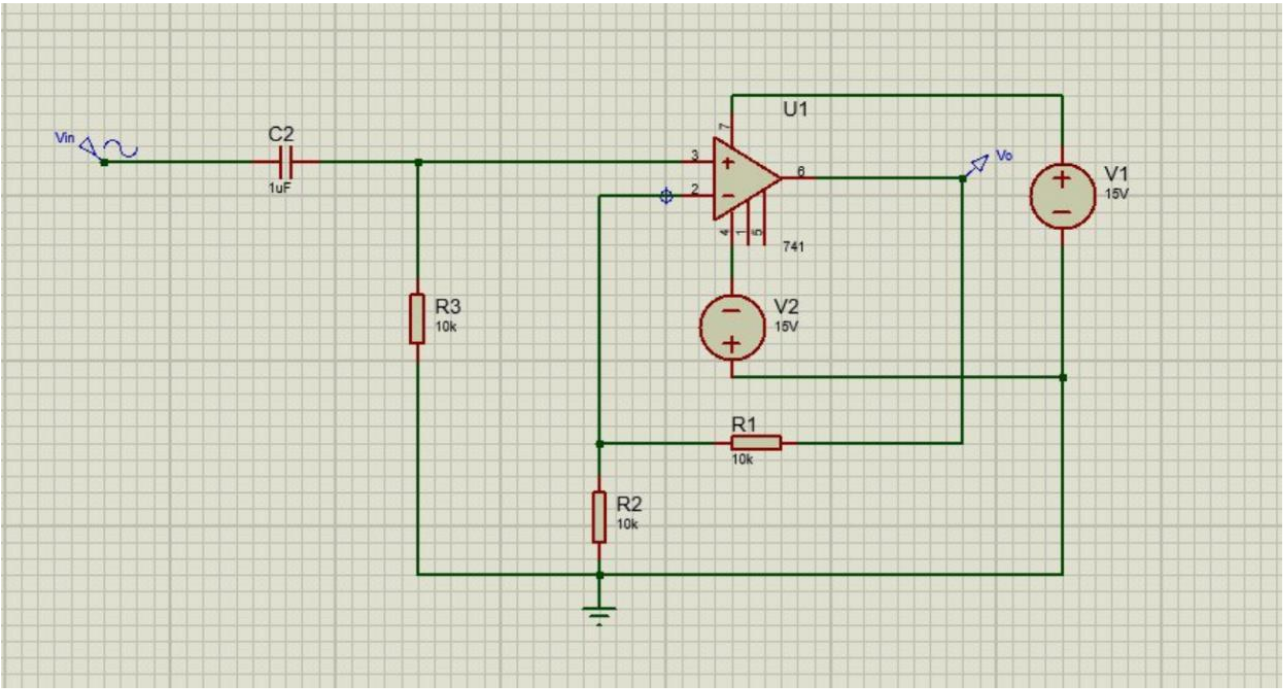
\includegraphics[width=0.8\textwidth]{HPF.png}
    \caption{High Pass Filter Circuit}
\end{figure}

\section{Result Analysis}

\subsection{Data Table}
A filter which passes only those signals whose frequencies are higher than cutoff frequencies thereby attenuating signals of lower frequencies. The value of cutoff frequency depends on the design of the filter. \\~\\

The basic High Pass Filter is built by a series connection of capacitor and resistor. While the input signal is applied to the capacitor, the output is drawn across the resistor. \\~\\

When we talk about cut of frequency we refer to the point in the frequency response in filter,where the gain is equal to 50\% the peak gain of the signal .i.e. 3dB of the peak gain. In High Pass Filter gain increases with an increase in frequencies.

\begin{table}[htpb]
    \centering
    \caption{Practical Data of High Pass Filter}
    \begin{tabular}{ccrc}
        \hline
        Vin &  Vout & Freuency & Av         \\
        \hline          
        1 & 0.019   &        1 & -34.424928  \\
        1 & 0.045   &        2 & -26.935750  \\
        1 & 0.113   &        3 & -18.938431  \\
        1 & 0.550   &        4 &  -5.192746  \\
        1 & 0.835   &        5 &  -1.566270  \\
        1 & 0.920   &        8 &  -0.724243  \\
        1 & 0.994   &       10 &  -0.052272  \\
        1 & 1.070   &       12 &   0.587676  \\
        1 & 1.140   &       15 &   1.138097  \\
        1 & 1.250   &       20 &   1.938200  \\
        1 & 1.310   &       25 &   2.345426  \\
        1 & 1.360   &       30 &   2.670778  \\
        1 & 1.400   &       40 &   2.922561  \\
        1 & 1.430   &       50 &   3.106721  \\
        1 & 1.460   &       75 &   3.287057  \\
        1 & 1.470   &      100 &   3.346347  \\
        1 & 1.480   &      150 &   3.405234  \\
        1 & 1.480   &      200 &   3.405234  \\
        1 & 1.490   &      300 &   3.463725  \\
        1 & 1.490   &      500 &   3.463725  \\
        1 & 1.490   &     1000 &   3.463725  \\
        1 & 1.480   &     2000 &   3.405234  \\
        1 & 1.480   &     3000 &   3.405234  \\
        1 & 1.480   &     5000 &   3.405234  \\
        1 & 1.430   &    10000 &   3.106721  \\
        \hline
    \end{tabular}
\end{table}

\newpage
\subsection{Graph}

\begin{figure}[h]
    \centering
    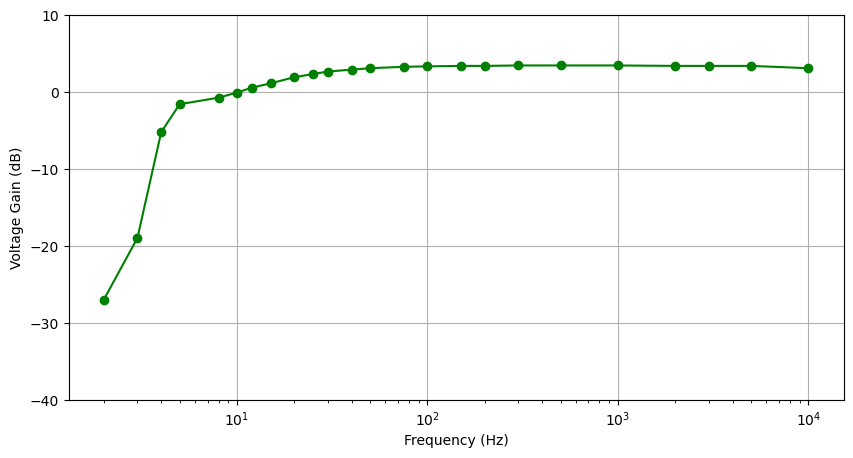
\includegraphics[width=0.8\textwidth]{HPF_Graph.png}
    \caption{Frequency Response of High Pass Filter}
\end{figure}

In this graph we were seen that at the low frequency the the gain was zero.After increasing the frequency randomly we were seen that this graph block the lower frequency and pass the higher frequency,and that was the condition of High Pass Filter.

\section{Discussion}
In this experiment we were seen that the High Pass Filter block the lower frequency and pass the higher frequency. The cut off frequency of the High Pass Filter was 1000Hz. The gain of the High Pass Filter was 3.463725. The gain of the High Pass Filter was increased with the increase of the frequency.

\end{document}

